\section{Implementation}

\begin{figure}
  \center
    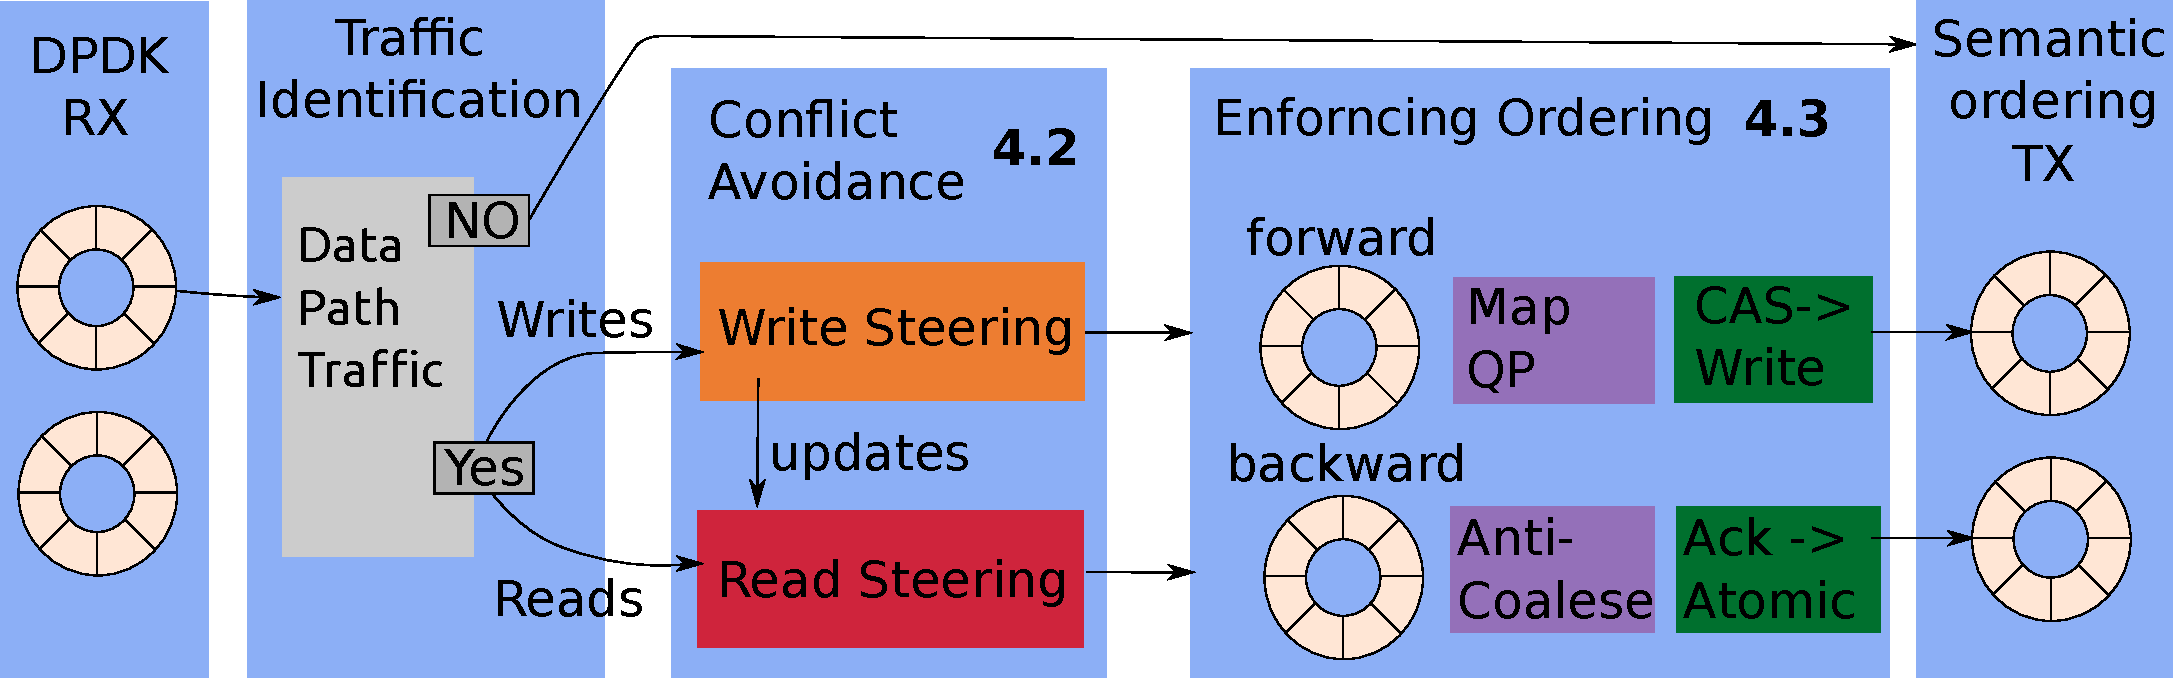
\includegraphics[width=0.45\textwidth]{fig/packet_processing.pdf}
    \caption{\sword's packet processing pipeline}
    \label{fig:system}
  \vskip -0.5em
\end{figure}

Our {\sword} prototype is implemented in P4 and run on a 100Gbps 64 port
programmable switch. Our P4 implementation includes the logic for identifying
and tracking connections, and resolving read and write conflicts in Clover.
Connection multiplexing is implemented separately on a DPDK middlebox discussed
further in this section.

\subsection{P4 implementation}

P4 is a highly constrained language. For example it does not support loops.
Architecturally P4 switches are also highly constrained. Packet parsing must be
performed using the limited TCAM resources available on the switch, conditionals
have a limited branching factor (4). Packets are processed in stages, and device
memory from one stage cannot be accessed at the next, therefore branching
conditionals which access the same variables must be aligned to the same switch
stage if they are to read or write to the same variables. In this section we
describe our P4 implementation of {\sword} and how it adheres to the constraints
of P4 and programmable switches.

\textbf{Parsing} {\sword} has no special requirements for packet parsing. Our
design is focused on RoCEv2 which runs over UDP. Our prototype implements
Ethernet, IP, UDP and RoCEV2 parsing. RoCEv2 headers are required for reading,
and manipulating virtual addresses. One additional header is required for Clover
to read the key out of write requests.

\textbf{Resource Utilization} {\sword} requires SRAM to cache data structure
information. The amount of data required is dependent on the data structure
itself. In clover we cache the last virtual address of each key, and we keep a
cache 3x the size of the keyspace for read steering.


\textbf{Traffic identification} Depending on the disaggregated
rack architecture, memory traffic might be coresident with regular
network traffic.  Additionally some of the traffic on the memory bus
may not require tracking or manipulation. In the case of Clover we do
not interpose upon or modify traffic to the metadata server as it is
not in the read/write path. The first stage of our packet-processing
pipeline classifies requests for manipulation. In our design operators
submit a filter as part of their configuration to allow traffic which does
not need to be modified to flow freely.

\textbf{Dynamic connection tracking}
 A key goal of our approach is to support
serializer-based performance enhancements without modifying the far memory
system itself---including requiring any explicit negotiation with the
serializer.  We add and subtract RoCE connections to {\sword}'s management
tables based upon the send and receipt of CAS operations. The QP and sequence
number for the CAS are stored on send, and the ATOMIC ACK is used to obtain the
other recever's QP.  As this approach requires only a single packet, requests
can be added and removed from our algorithm dynamically with little effort.

%For instance is designed to deal with memory operations made to the wrong
%location via iterative pointer chasing. We strongly suggest that disaggregated
%algorithms take this approach as our middlebox solution only acts to acclerate
%operations in the common case.
\textbf{Initializing connection mapping}
\sg{dpdk only}
As some state may be dependent on the number of connections (such as the
key-to-QP and lock-to-QP mappings), state transitions either require a lock, or
the copying of current state over to a new epoch when new connections are added.
In all of our experiments only one such transition is made. We begin our mapping
after a specific number of clients for the experiment have connected. Once the
total number of clients have connected, a switch is flipped, and the QP
multiplexing algorithm begins. Requests which do not have mappings stored, but
were in flight during the flip have their sequence numbers and MSN values
applied to the connection state of the new epoch.

%\subsection{Operation caching}
%\label{sec:operation-caching}



% \begin{figure}
%     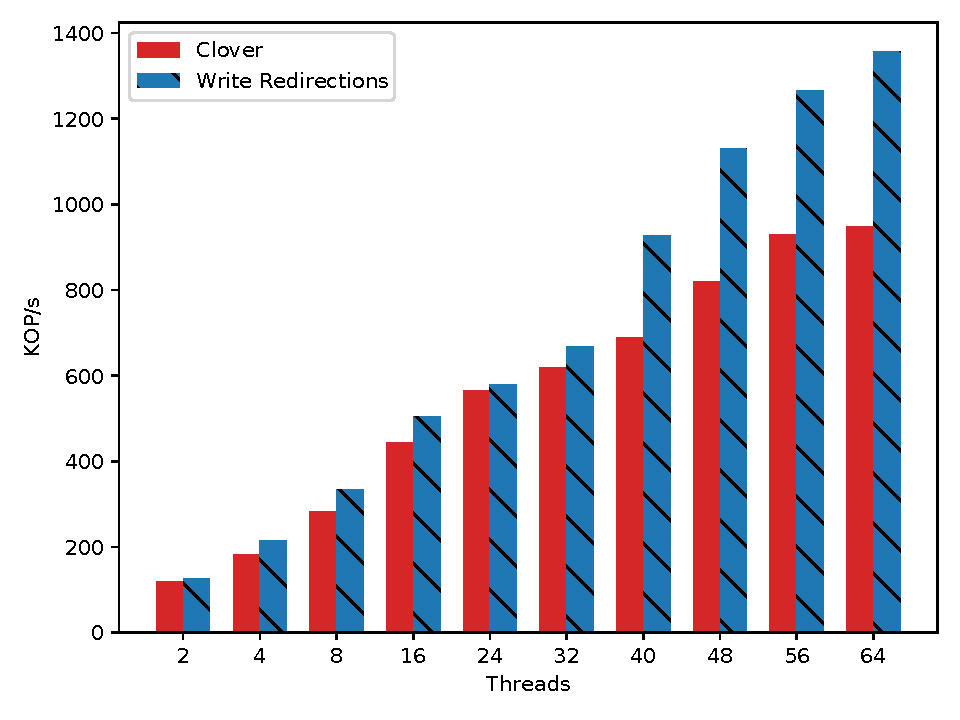
\includegraphics[width=0.45\textwidth]{fig/throughput.pdf}
%     \caption{Default Clover throughput vs. Clover with write conflict
%     detection and correction turned on \todo{recompute with the read caching values (old)}}
%     \label{fig:throughput}
%     \vskip -1em
% \end{figure}

% \subsection{Implementing Atomic replacement}

% In the
% following subsections we describe the dangers of removing atomics, and present
% our solutions.

% A few assumptions must be made in order for this replacement of operations to be
% made. First and foremost all operation serialization must be made, and finalized
% at the point where the CAS is swapped out. More formally, all of the data
% structure invariants which required locking, must be satisfied at the time of
% transforming the packet. Further the order of operations must be maintained
% downstream from the checking of the invariant. These two requirements influence
% the design of any system which aims to make this performance improvement.


%% ACS - This is just lifted from WORDS; no need to repeat here

%% \begin{figure}
%%     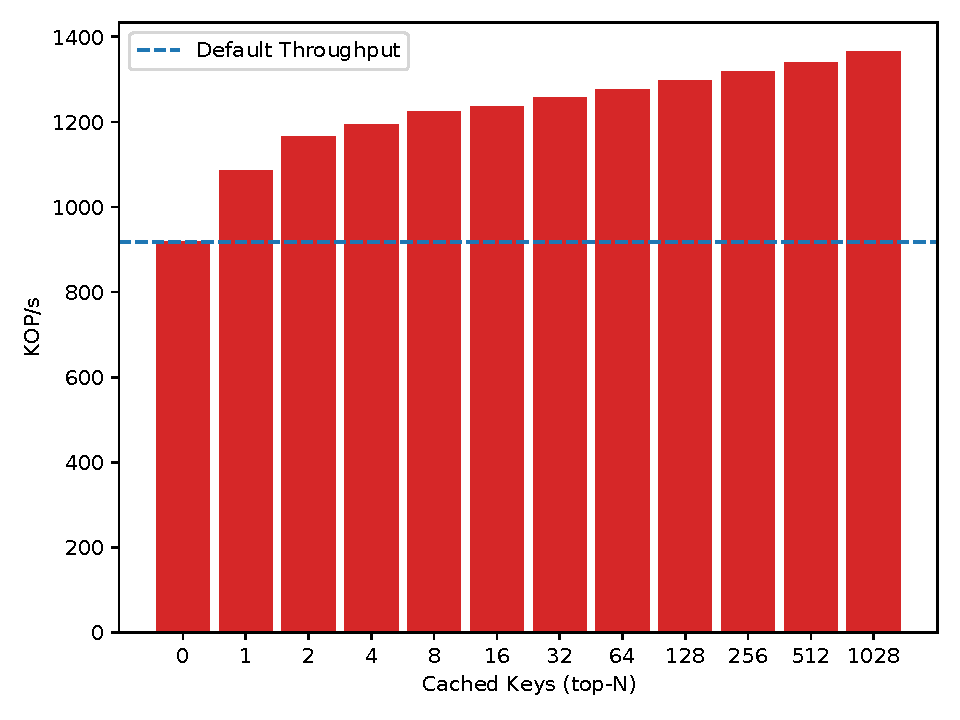
\includegraphics[width=0.45\textwidth]{fig/cache.pdf}
%%     \caption{Performance as a function of keys cached. Caching a few
%%     of the top-$N$ keys provides the greatest marginal throughput
%%     benefits.}
%%     \label{fig:cache}
%% \end{figure}

%% \textbf{reduced cache size} we show that if hot keys are known we require only a
%% small amount of in network state~\ref{fig:cache} we have considered dynamic
%% approaches such as LRU which would allows for a finite amount of space and an
%% arbitrary number of keys to be serviced.

% The first requirement, that the structural invariants
% of the data structure be maintained at the point of transformation demands that
% all of the state required to check the structural invariant be present at the
% point in the network at which the swap is made. This fact increases the memory
% cost on a switch, however with intelligent data structure design the cost of the
% required metadata can be mitigated. In the case of Clover, while each key has
% an entire linked list history that can potentially span megabytes, the only
% required metadata to make the change from CAS to write is the location of the
% tail pointer. In this case the metadata cost is O(n) as it grows linearly with
% the keyspace.

% \textbf{2) reordering} The second requirement, that operations not be reordered
% after the invariant has been checked requires more care in real systems. For
% instance in an RDMA system with two clients, both could have contesting CAS
% operations swapped with writes. As the two clients are transmitting operations on
% separate QP, and the receiving NIC makes no guarantees about ordering between QP,
% the operations could easily be reordered. In the case with CAS, the order could
% be forced by ensuring that if one write was to succeed the second would fail.
% Without this guarantee the preservation of operation ordering must be maintained
% in another way.

% \subsection{Connection Remapping}


% Our solution here is simple, given that we have the key's for reads and writes
% (Section ~\ref{sec:operation-caching}), all operations for the same key are
% mapped to the same QP.  This algorithm requires that a few pieces of state be
% maintained per connection.  First the sending and response QP for each sender
% and receiver need to be tracked. Second the sequence number of each connection,
% and the original message sequence number offset must be maintained. Per client
% connection the pair of QP's require 48 bits, and the sequence + message sequence
% require an additional 48 for a total of 12 bytes per connection. The storage
% requirement for mapped requests varies based on the algorithm. If clients are
% able to issue an unbounded number of async requests, then a buffer large enough
% to maintain backwards mappings for each request is required. In clover clients
% can issue up to 2 async requests, so we keep a two 6 byte mappings for each
% connection available to map back. 

% Depending on the algorithm and the QP mapping scheme requests from a single
% sender can be reordered. That is, if a client makes a read and write request to
% different locations in memory, and they are mapped to different QP, they may be
% returned out of order. Infiniband allows for out of order operations on
% receivers~\cite{infiniband-spec}, which pushes operation ordering to client
% side user space. Roce does not allow for out of order operations. In this case
% the receiving NIC will retransmit if requests are delivered out of order. Here
% we buffer requests in network, as we have application knowledge the size of the
% buffer is bounded (to the size of a single read packet in clovers case). We
% suggest that given the tight memory restrictions on middleboxes algorithms which
% have an unbounded number of async requests leave the ordering of remapped
% requests to client side user space using IB verbs or a different transport layer
% entirely.

\subsection{RDMA ICRC}

RDMA requests are not intended to be modified in flight, and care must
be taken not to corrupt them. RDMA invariant CRCs (ICRC) are
calculated at the time of sending and are designed to ensure the
integrity of the payload. When we modify requests their ICRC must be
recalculated or the packet will be rejected by the receiving NIC. Such
an error would cause an extreme performance hit as any dropped packet
triggers a timeout, and go back n retransmission.  FPGA
implementations of RDMA ICRC have been built in the
past~\cite{Mansour_2019}; the required CRC calculation is identical to
Ethernet CRC, with some additional \texttt{crc32} for the
calculation. This algorithm is highly optimized for general case CRC
calcuation.

Recalculating the CRC for modified requests is the primary overhead of {\sword}
as it must be recalculated after a squence number update, which occurs on all
multiplexed and demultiplexed requests. This overhead could be reduced by either
removing the need for the CRC (which is not a feature available on CX series
NICs) or by allowing an alterative, lightweight checksum which could be quickly
updated based on changes made to the packet while in flight. While these options
are not currently available we believe that commodity switches and SmartNICs
could leverage hardware offloads to reduce the cost, as the CRC calculation is
identical to Ethernet with only the additional need to mask RocE specified
packet felids.

We implemented RDMA ICRC in our DPDK prototype. To our knowledge no P4 switches
have native RoCEv2 support, while some projects have demonstrated that it is
possible to implement by hand, it requires many switch resources and adds
complexity~\todo{~\cite{}} we forgot the additional complexity and turned off
ICRC checking on our CX5 NICs similar to prior work~\cite{switchml}. In the
future we hope that RoCEv2 checksums, like TCP, UDP,and Ethernet checksums can
be made hardware primitives on programmable switches.

\subsection{DPDK considerations}

{\sword} is implemented in DPDK for ease of programmability, but
requires that all requests are processed without the aid of RDMA
hardware on the NIC. Using DPDK introduces issues in terms of
performance as individual cores on the server have low packet
processing capabilities relative to dedicated networking hardware. As
such our design is multithreaded and requires the use of careful
atomics for performance.  Our design partitions cores into TX and RX
groups. RX cores are configured via RSS and perform traffic
identification, write steering and mapping. We completely removed the
need for any explicit locking between cores and share as little state
as is theoretically possible. Each TX core serializes requests by
making atomic fetch-and-add updates to a shared region of memory
containing connection sequence and message-sequence numbers. RX cores
are handed packets from TX cores using DPDKs lock-less ring
library. TX cores check packets to determine if they require CRC
computation and calculate the CRC only if the packet has been
modified. Adding a packet handoff between TX and RX increases latency,
however the head-of-line blocking incurred by having a single core
perform both mapping and CRC calculations is too high for our purposes.

We find that by using an array size of
3$\times$ the vast majority of reads succeed first try.
%One advantage
%of this technique is that it is a generalized cache for recent RDMA
%reads, and requires little computation to maintain a hot cache.
For
performance reasons we forgo heavyweight hash functions and use
the \texttt{murmur3} bit scrambler to attain an approximately even
hash of virtual addresses in only a few cycles.
%---which can likely be
%implemented on programable switch hardware.



